\documentclass[letter,12pt]{article}

\usepackage[T1]{fontenc}
\usepackage[utf8x]{inputenc}
\usepackage{fullpage}

\usepackage{tikz-uml}
\begin{document}
\thispagestyle{empty} 
\begin{figure}[!ht]
\begin{center}
\hspace*{-50pt}
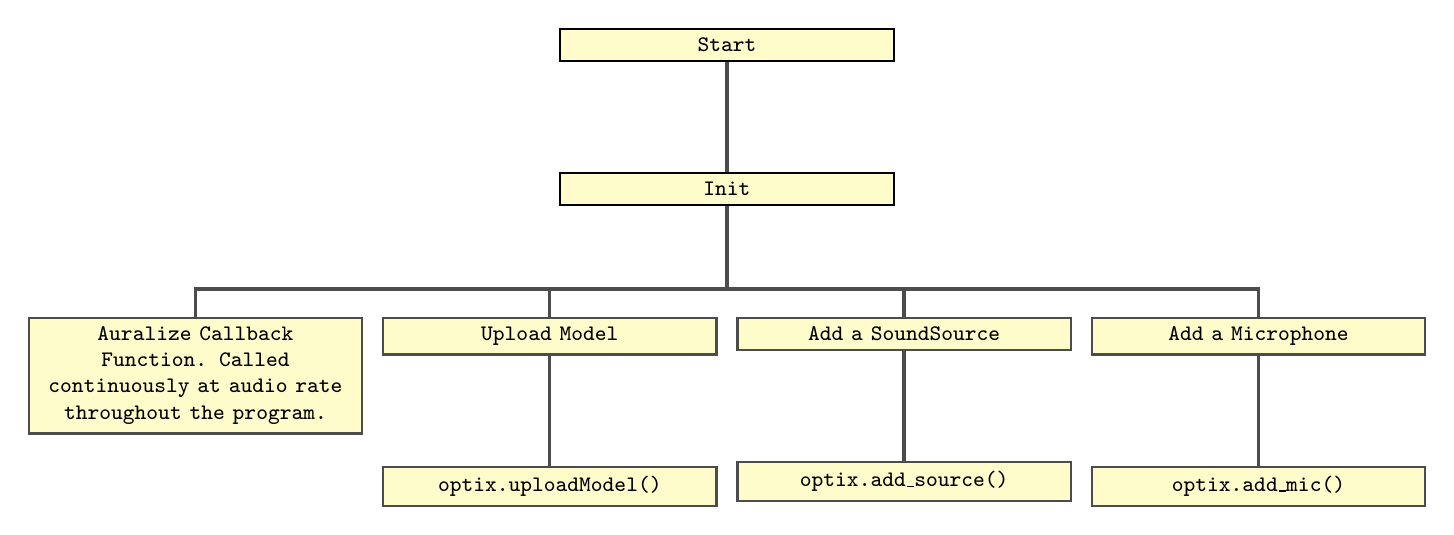
\begin{tikzpicture}[
% Label style
    label distance=3mm,
    every label/.style={blue},
% Event style
    event/.style={rectangle,thick,draw,fill=yellow!20,text width=4cm,
		text centered,, font=\footnotesize\ttfamily,anchor=north},
% Children and edges style
    edge from parent/.style={very thick,draw=black!70},
    edge from parent path={(\tikzparentnode.south) -- ++(0,-1.05cm)
			-| (\tikzchildnode.north)},
    level 1/.style={sibling distance=3cm,level distance=1.4cm,
			growth parent anchor=south,nodes=event},
    level 2/.style={sibling distance=4.5cm},
    level 3/.style={sibling distance=4cm},
    level 4/.style={sibling distance=4cm}
%%  For compatability with PGF CVS add the absolute option:
%   absolute
    ]
   \node [event] {Start}
	     child{node {Init}   
	     	child {node {Auralize Callback Function. Called continuously at audio rate throughout the program.}}
	     	child {node {Upload Model}
	     	   child {node {optix.uploadModel()}}
	     	}
	     	child {node {Add a SoundSource}
	     	    child {node{optix.add\_source()}}
	     	}
	     	child {node {Add a Microphone}
	     	    child {node {optix.add\_mic()}}
	     	}
		};
	     	   
\end{tikzpicture}
\vspace{.15in}
\end{center}
\end{figure}
\end{document}